\section{Estimation of liquid water production at the test bench}
% by Christian Kunde
% christian.kunde@ovgu.de / kunde@mpi-magdeburg.mpg.de
%
%
\subsection{Estimation from test bench measurements}
%
The rate of liquid water produced in the stack can be estimated from test bench measurements.
%
\begin{itemize}
   %%%
   \item \highlightg{additional assumptions}
     \begin{itemize}
        \item steady state
        \item constant environment conditions
%         \item coolant flow $F_\vl{cool}=\text{constant}$ % only for signal shift in MATLAB file
        \item no diffusion or drag through the membrane
        \item no short circuit currents
        \item no side reactions
        \item stack perfectly insulated
        \item kinetic energy can be neglected
        \item no liquid water enters the stack
     \end{itemize}
   %%%
   \item \highlightg{gas humidification to a set dew point temperature}\\ Increase water vapor content of a dry gas flow up to a specified dew point temperature, where the dew point is the temperature at which the gas would be saturated with water vapor, \ie
        \begin{align}
         p_\vl{H_2O}=p_\vl{H_2O}^\vl{\ast}(T_\vl{d})
        \end{align}
       where $T_\vl{d}$ is the dew point temperature, $p_\vl{H_2O}$ is the partial pressure of water vapor, and $p_\vl{H_2O}^\vl{\ast}$ is the saturation vapor pressure.\\
       The saturation vapor pressure is approximated by
%        
       \begin{align}
        p_\vl{H_2O}^\vl{\ast}(T_\vl{d}) = 100\,\vl{Pa}\, \eu^{19.016 - \frac{4064.95 }{ T_\vl{d}/\vl{K} - 273.15 + 236.25}}.
       \end{align}
% 
       In an ideal gas mixture
        \begin{align}
         \frac{p_\vl{H_2O}}{p} = \frac{n_\vl{H_2O}}{n} \quad\Rightarrow\quad \frac{p_\vl{H_2O}}{p} = \frac{\dot{\tilde n}_\vl{H_2O}}{\dot{\tilde n}}
        \end{align}
       where $n$ are mole amounts, $p$ is the total pressure, $\dot{\tilde n}$ is the total humidified molar flow, and $\dot{\tilde n}_\vl{H_2O}$ is the water vapor molar flow.\\
       Therefore, with the dry gas molar flow $\dot{\tilde n}_\vl{dry}$,
        \begin{align}
         \frac{p_\vl{H_2O}}{p} &= \frac{\dot{\tilde n}_\vl{H_2O}}{\dot{\tilde n}_\vl{H_2O} + \dot{\tilde n}_\vl{dry}}\\
          &\Downarrow \quad \nonumber\\
         \dot{\tilde n}_\vl{H_2O} &= \frac{p_\vl{H_2O}}{p-p_\vl{H_2O}} \dot{\tilde n}_\vl{dry} \\
          &\Downarrow \quad p_\vl{H_2O}=p_\vl{H_2O}^\vl{\ast}(T_\vl{d}) \nonumber\\
         \dot{\tilde n}_\vl{H_2O} &= \frac{p_\vl{H_2O}^\vl{\ast}(T_\vl{d})}{p-p_\vl{H_2O}^\vl{\ast}(T_\vl{d})} \dot{\tilde n}_\vl{dry}
        \end{align}
   %%%
   \item \highlightg{mass balances total stack including reaction}\\
       Molar flows at the stack outlets can be calculated from mass balances and the measured stack current:
       \begin{align}
         \dot{\tilde n}_\vl{O_2,c,out} &= \dot{\tilde n}_\vl{O_2,c,in}  - \frac{I_\vl{S}}{4 \vl{F}}  N_\vl{cells} \\
         \dot{\tilde n}_\vl{N_2,c,out} &= \dot{\tilde n}_\vl{N_2,c,in} \\
         \dot{\tilde n}_\vl{H_2O,c,out} &= \dot{\tilde n}_\vl{H_2O,c,in}  + \frac{I_\vl{S}}{2 \vl{F}}  N_\vl{cells} \\
         \dot{\tilde n}_\vl{H_2O,a,out} &= \dot{\tilde n}_\vl{H_2O,a,in}\\
         \dot{\tilde n}_\vl{H_2,a,out} &= \dot{\tilde n}_\vl{H_2,a,in}  - \frac{I_\vl{S}}{2 \vl{F}}  N_\vl{cells} 
       \end{align}
       %
       where $\dot{\tilde n}$ are molar flows, $I_\vl{S}$ is the stack current, $N_\vl{cells}$ is the number of cells in the stack, and $\vl{F}$ is the Faraday constant.
   %%%
   \item \highlightg{maximum transport capacity of water vapor at stack outlets}\\
       The maximum capacity is reached when the outlet gas flow is fully saturated with water vapor, \ie
        \begin{align}
         p_\vl{H_2O,out,max}&=p_\vl{H_2O}^\vl{\ast}(T_\vl{out})\\
          &\Downarrow \quad \nonumber\\
         \frac{\dot{\tilde n}_\vl{H_2O(g),out,max}}{\dot{\tilde n}_\vl{H_2O(g),out,max}+\dot{\tilde n}_\vl{dry,out}} p_\vl{out}&=p_\vl{H_2O}^\vl{\ast}(T_\vl{out})         
        \end{align}
       where $p_\vl{out}$ is the total pressure at the outlet and $\dot{\tilde n}_\vl{dry,out}$ is the molar flow at the outlet excluding $\vl{H_2O}$.\\
       Solving for $\dot{\tilde n}_\vl{H_2O,out,max}$ gives the maximum transport capacity of water vapor at the stack outlets:
        \begin{align}
         \dot{\tilde n}_\vl{H_2O(g),out,max} = \frac{p_\vl{H_2O}^\vl{\ast}(T_\vl{out})}{p_\vl{out}-p_\vl{H_2O}^\vl{\ast}(T_\vl{out})} \dot{\tilde n}_\vl{dry,out}   
        \end{align}
   %%%
   \item \highlightg{water vapor and liquid water at the stack outlets}\\
       %
       Assuming all liquid water is evaporated until the gas is fully saturated, we get
        \begin{align}
         \dot{\tilde n}_\vl{H_2O(l),out} &= \max(0,\dot{\tilde n}_\vl{H_2O(g),out}-\dot{\tilde n}_\vl{H_2O,out,max}),\\
         \dot{\tilde n}_\vl{H_2O(g),out} &= \min(\dot{\tilde n}_\vl{H_2O(g),out},\dot{\tilde n}_\vl{H_2O,out,max}),
        \end{align}
       where $\dot{\tilde n}_\vl{H_2O(l),out}$ is the liquid water molar flow at the outlet and  $\dot{\tilde n}_\vl{H_2O(g),out}$ is the water vapor molar flow at the outlet.
   %%%
\end{itemize}
%
%
\subsection{Validation via overall energy balance}
%
An overall energy balance for the fuel cell stack can be used to validate the assumptions for the calculation of the liquid water production.
Including liquid water in the considerations gives much better results for the energy balance, both qualitatively and quantitatively, than neglecting liquid water production.
This suggest that the assumptions for calculation the production rate of liquid water fit the test bench setup sufficiently well.
%
\begin{itemize}
    %%%
    \item \highlightg{energy balance}\\
        The energy balance for the total stack comprises the energy transported by mass flows \eqref{eqn-edot}, the mechanical work done on/by the system \eqref{eqn-Psurf1}-\eqref{eqn-Psurf3}, the heat transported by cooling water \eqref{eqn-Wcool}, and the electrical work done by the system \eqref{eqn-Wel}.\\
        The steady-state equation simplifies to
         \begin{align}
         0 = &\quad\sum\limits_{i_\vl{c}} \left( \dot{\tilde n}_{i_\vl{c},\vl{in,c}} e_{i_\vl{c},\vl{in,c}} - \dot{\tilde n}_{i_\vl{c},\vl{out,c}} e_{i_\vl{c},\vl{out,c}} + \dot{\tilde n}_{i_\vl{c},\vl{in,a}} e_{i_\vl{c},\vl{in,a}} - \dot{\tilde n}_{i_\vl{c},\vl{out,a}} e_{i_\vl{c},\vl{out,a}} \right) \label{eqn-edot}\\
             &+ \dot{\tilde n}_\vl{in,c} \vl{R} T_\vl{in,c} - \dot{\tilde n}_\vl{out,c} \vl{R} T_\vl{out,c}
              + \dot{\tilde n}_\vl{in,a} \vl{R} T_\vl{in,a} - \dot{\tilde n}_\vl{out,a} \vl{R} T_\vl{out,a} \label{eqn-Psurf1}\\
             &- \dot{\tilde n}_\vl{H_2O(l),out,a} p_\vl{H_2O,out,a} \frac{ M_\vl{H_2O}}{\varrho_\vl{H_2O}}
              - \dot{\tilde n}_\vl{H_2O(l),out,c} p_\vl{H_2O,out,c} \frac{ M_\vl{H_2O}}{\varrho_\vl{H_2O}}\label{eqn-Psurf3}\\
             &+ \dot{\tilde n}_\vl{H_2O,cool} c_\vl{p,H_2O} (T_\vl{in,cool}-T_\vl{out,cool}) \label{eqn-Wcool}\\
             &- I_\vl{S} U_\vl{S} \label{eqn-Wel}
        \end{align}
       where the specific energies $e$ are equal to specific internal ernergies $u$ for zero kinetic energy, and $i_\vl{c} \in \{\vl{H_2O(l)},\vl{H_2O(g)},\vl{N_2},\vl{O_2},\vl{H_2} \}$.\\
       The specific internal ernergies $u$ are calculated according to ideal gases for the gas flows and according to incompressible fluids for liquid water flow.
       \begin{align}
        &u_\vl{ideal\,gas} = h_\vl{ref}+\int\limits_{T_\vl{ref}}^T c_\vl{p}(\tau)\op{d}\tau - \vl{R} T\\
        &u_\vl{incompressible} = h_\vl{ref}+\int\limits_{T_\vl{ref}}^T c_\vl{p}(\tau)\op{d}\tau-\frac{p_\vl{ref} M}{\varrho_\vl{ref}}
       \end{align}
       Note that, for ideal gases, some expressions from surface work and internal energy cancel each other out.\\
       Here, $c_\vl{p}$ are heat capacities, $\dot{\tilde n}_\vl{H_2O,cool}$ is the molar flow of coolant water, $T_\vl{in/out,cool}$ are coolant temperatures at in-/outlet, $\dot{\tilde n}_\vl{in/out,a/c}$ are tolar molar gas flows, $\vl{R}$ is the universal gas constant, $M$ is the molar mass, and $U_\vl{S}$ is the stack voltage.
   %%%
   \item \highlightg{heat of condensation}\\
       %
       The additional heat available due to liquid water leaving the stack instead of vapor can be considered as an individual contribution to the energy balance:
       \begin{align}
        P_\vl{th,cond} := \dot{\tilde n}_\vl{H_2O(l),out,a}(h_\vl{H_2O(g),a}-h_\vl{H_2O(l),a}) + \dot{\tilde n}_\vl{H_2O(l),out,c} (h_\vl{H_2O(g),c}-h_\vl{H_2O(l),c})
       \end{align}
       Note that the stack energy balance only considers that liquid water leaves the stack, not whether it actually condenses or whether it might be produced directly as liquid water.
       %
   %%%
   \item \highlightg{graphical analysis}\\
       %
       The right-hand side of the energy balance equation should be close to zero.
       Some deviation due to the rough assumptions is expected.
       Note that spikes and extreme plateaus for the heat of condensation are due to faulty dew point measurements.
       Analyzing individual contributions to the energy balance seems to validate the calculations for the production rate of liquid water:\\
       \begin{center}
       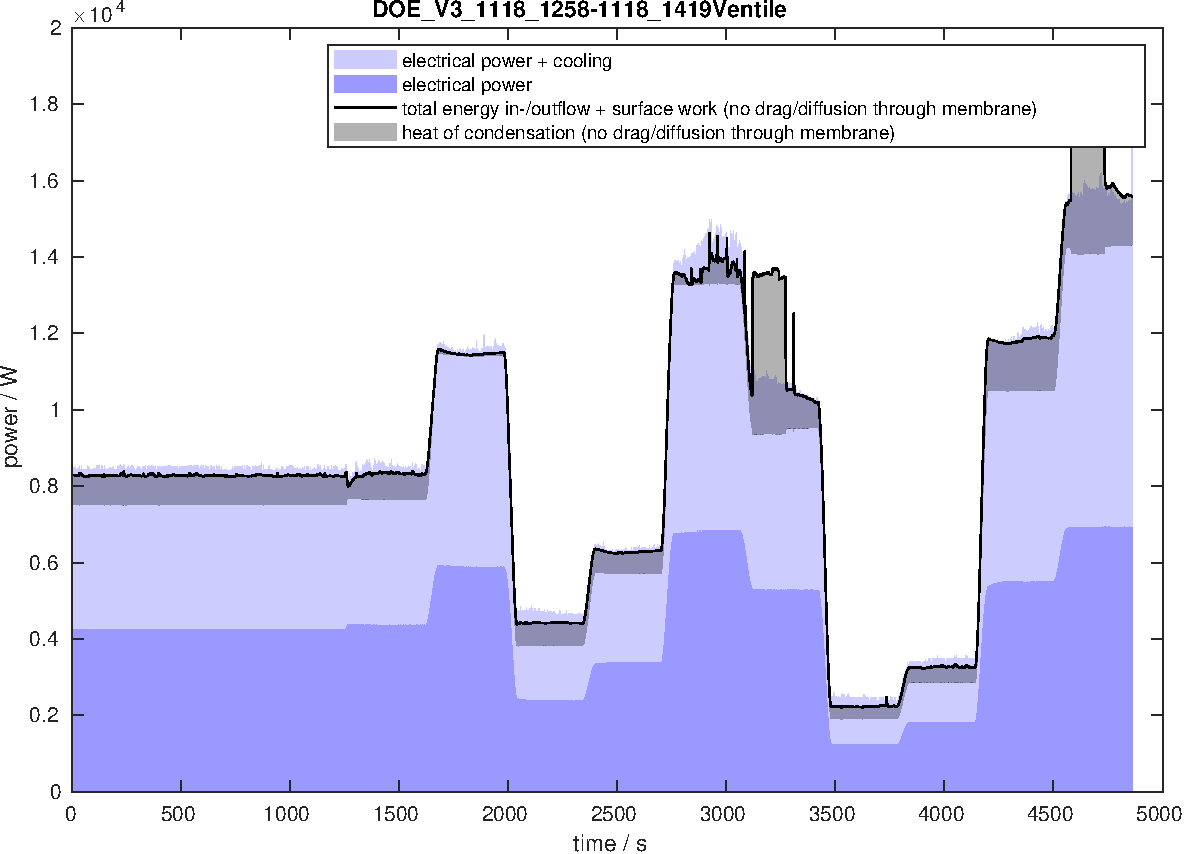
\includegraphics[scale=0.6]{./figures/energyBalance_DoE_v3}
       \end{center}
   %%%
\end{itemize}
%
%
\subsection{Estimation from test bench inputs}
%
If measuremsts from the test bench are not yet available, \eg for the design of a future experiment, the rate of liquid water production can be estimated from fuel cell stack inputs alone by making further assumptions.
The fuel cell voltage and the resulting stack outlet temperature as well as the gas pressures at the inlets are unknown in this case.
Depending on the available knowledge, the cooling outlet temperatures can be estimated from a simplified energy balance.\smallskip
%
\begin{itemize}
   %%%
   \item \highlightg{additional assumptions}
     \begin{itemize}
      \item cooling water and cathode gas in co-flow, anode gas in counter-flow
      \item gas temperatures approach cooling temperature at the gas outlets\\
            $T_\vl{out,c} \approx T_\vl{cool,out}$, $T_\vl{out,a} \approx T_\vl{cool,in}$
      \item options for $T_\vl{cool,out}$
        \begin{itemize} 
          \item $T_\vl{cool,out} \approx T_\vl{cool,in}$ (this overestimates condensation because ${T_\vl{cool,out}\ge T_\vl{cool,in}}$)
          \item assuming a fixed value for the average cell voltage $U_\vl{cell}=\text{constant}$
          \item assuming an average U-I curve for the cell voltage $U_\vl{cell}(I_\vl{cell})$
        \end{itemize}
      \item $p_\vl{in,a/c} \approx p_\vl{out,a/c}$
     \end{itemize}
   %%%
\end{itemize}
